Phần cứng máy tính nhúng được sử dụng là mạch phát triển Raspberry Pi 3 với sơ đồ ra chân như hình \ref{rpi3-pinout}. 
\begin{figure}[H]
	\centering
	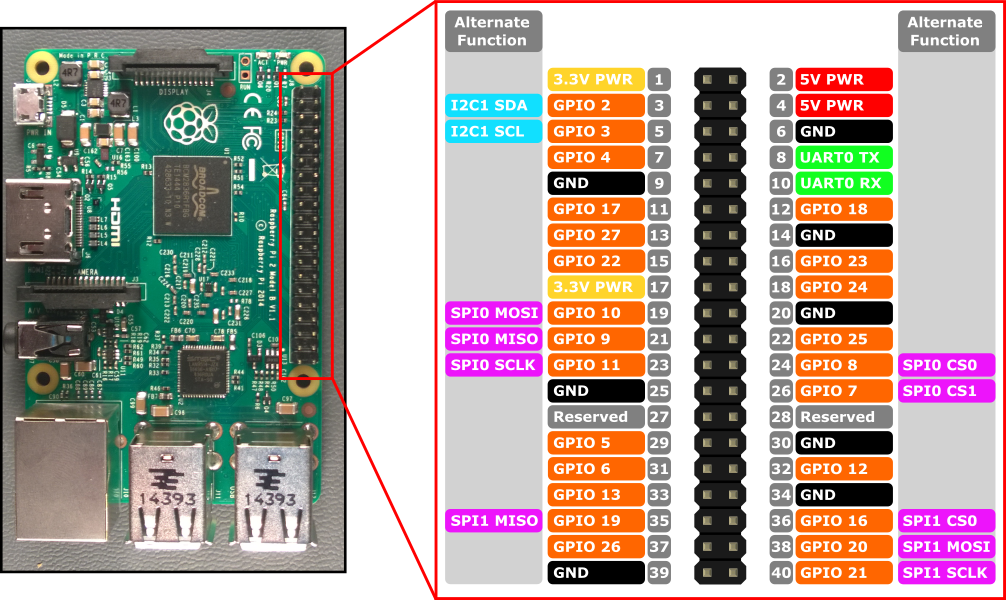
\includegraphics[width=0.8\textwidth]{../images/rp3_pinout.png}
	\caption{Sơ đồ ra chân các ngoại vi của Raspberry Pi}
	\label{rpi3-pinout}
\end{figure}

Mô đun PCF8574 cho màn hình LCD1602 được kết nối tới Raspberry Pi qua ngoại vi I2C1 duy nhất với 4 dây nối tương ứng trong bảng \ref{wiring}.

\begin{table}[H]
	\centering
	\caption{Sơ đồ nối dây giữa Raspberry Pi và mô đun PCF8574}
	\begin{tabular}{|c|c|}
		\hline
		\textbf{Chân Raspberyr Pi} & \textbf{Chân PCF8574}\\
		\hline
		5V & VCC\\
		GND & GND\\
		GPIO3 & SCL\\
		GPIO2 & SDA\\
		\hline
	\end{tabular}
	\label{wiring}
\end{table}
